\section{Äquivalenzrelationen}

\subsection{Bemerkung:}
	Es sei $f: A \rightarrow B$ eine Abbildung. Für jedes feste $b \in B$ nennen wir $f^{-}(b) = \{ a \in A | f(a) = b\}$ die Faster von $b$ unter $f$. Offenbar sind je zwei Fasern disjunkt: $b_{1} \neq b_{2} \Longrightarrow f^{-} (b_{1}) \cap j(b_{2}) = \emptyset$ ferner ist $ A =  	\bigcup_{b \in B} j(b)$. Wir sprechen von einer disjunkten Zerlegung bzw. Partition von $A$. /*  Faser $\mathrel{\widehat{=}}$ volles Urbild; disjunkt = Schnitt ist leer. */ 

\subsection{Beispiel:}
	$ A =$ Menge aller Autos. \\
	$ F =$ Menge aller Farbcodes von Autos.\\
	$f: A \rightarrow F$ ordnet jedem Auto seinen Farbcode zu. Damit werde die Autos andhand ihrer Farbe ( Faser von blaue ( blaue Autos)) in unterschiedliche Schubladen gepackt, die Faser von $f$. Die Fasern sind disjunkt, da jedes Auto einen bestimmten Farbcode hat. Jedes Auto hat einen Farbcode, liegt also in einer Faser. \\
Vermöge $f$ können zwei Autos gleicher Farbe als "`gleichwertig"' angesehen werden. 

\subsection{Definition:}
Eine Äquivalenzrelation auf einer Menge $A$ sei eine Teilmenge von $!_{R}$ von $A$x$A$ mit folgenden Eigenschaften:
\begin{description}

	\item[R ist refelxiv:] für jedes $a \in A$ ist $(a,a) \in $ R
	\item[R ist symmetrisch:] ist $(a_{1}, a_{2}) \in $ R, so auch $(a_{2},a_{1}) \in$ R
	\item[R ist transitiv:] sind $(a_{1}, a_{2}),(a_{2}, a_{3}) \in$ R, so auch $(a_{1},a_{3}) \in$ R

\end{description}
Anstatt $(a,b) \in$ R schreiben wir $a \sim_{R} b$ und sagen "`a äquivalent b"'.

\subsection{Beispiel:}

  \begin{enumerate}[label={\alph*)}]
     \item zu Beispiel 2.2 ist $\mathbb{R} = \{ (a,b) \in A$x$A|f(a) = f(b)\}$ eine Äquivalenzrelation auf der Menge $A$ aller Autos. 
     \item Auf jede Menge ist die Gleichheit "`="' von Elmenten eine Äquivalenzrelation. 
	\item Kongruenz von Dreiecken in der Zeichenebene $R^{2}$ ist eine Äquivalenzrelation auf der Menge dieser Dreiecke.
  \end{enumerate} 
%
%
%
\subsubsection{Erinnerung}
	Äquivalenzrelation $\sim$ auf $M$
\begin{description}
	\item [-] reflexiv $\forall a \in M a \sim a$
	\item [-] symmetrisch wenn $ a \sim b$, dann $b \sim a$
	\item [-] transitiv wenn $a \sim b \wedge b \sim c$, dann $a \sim c$
\end{description}
%
%
%
\subsection{Definition:}

Es sei $\sim$ eine Äquivalenzrelation auf $M$. Für jede \\
$a \in M$ sei $\{ b \in M | a \sim b\} = [a] =_{wegen Symmetrie} \{b \in M | b\sim a\}$ die sogenannte \underline{Äquivalenzklasse} zu a. \\
Jedes $b \in [a]$ heiße ein \underline{Vertreter} von $[a]$. 
\begin{description}
	\item[\underline{Beachte:}] Reflexivität $\Rightarrow a$ Vertreter von $[a]$ (wegen Symmetrie).
\end{description}
%
%
%
\subsection{Hauptsatz:}
Es sei $M$ eine feste Menge. Dann gilt:
\begin{description}
	\item[-] Die Äquivalenzrelationen auf $M$ entsprechen genau den Partitionen von $M$.
\end{description}
Genauer:
\begin{description}
	\item[(a)] Ist $M = \dot{\bigcup}_{i \in I}$ $M_{i}$ ($\dot{\bigcup}$  = disjunkte Vereinigung) eine Partition von $M$, so ist eine Äquivalenzrelation $\sim$ auf $M$ gegeben durch: $a \sim b \Leftrightarrow$ es gibt ein $i \in I$ mit $a,b \in M_{i}$ Die Äquivalenzklassen zu $\sim$ sind genau die Mengen $M_{i} (i \in I)$
	\item[(b)] Ist $\sim$ eine Äquivalenzrelation auf $M$, so bilden die 'quivalenzklassen zu $\sim$ eine Partition von M.
	\item[(c)] Die durch $(a)$ und $(b)$ gegebenen Abbildungen sind bijektiv und gegenseitig invers. 
		\begin{figure} [H]
		\centering 
		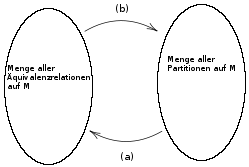
\includegraphics[width=8cm, height=5cm]{mainmatter/chapter1/pics/bijektivinvers.png}
		\caption{Eine bijektive und inverse Abbildung} 
		\end{figure}
\end{description}
%
%
%
\subsubsection{Beweis:}
\begin{description}
	\item[(a)] \quad
	\begin{description}
		\item[\underline{reflexiv:}] Sei $a \in M$. Dann existiert ein $i \in I$ mit $a \in M_{i} \Rightarrow a \sim a$.
		\item[\underline{symmetrisch:}] Seien $a,b \in M$ mit $a \sim b \Rightarrow \exists i \in I: a,b \in M_{i} \Rightarrow b \sim a$.
		\item[\underline{transitiv:}] Seien $a,b,c \in M$ mit $a \sim b$ und $b \sim c \Rightarrow$ es gibt $i \in I$ mit 
			$a,b \in M_{i}$ und es gibt $j\in J$ mit $b,c \in M_{j}$ Da $b \in M_{i} \wedge M_{j}$ und die Partition $M 
			= \dot{\bigcup}_{i \in I} M_{i}$ disjunkt ist, ist $i = j \Rightarrow a,c \in M_{i} = M_{j}$ und somit $a \sim 
			c$. Nach Definition von $\sim$ ist $[a] = M_{i}$ für das einzige $i \in I$ mit $a \in M_{i}$
	\end{description}
	\item[(b)] Jeder $a \in M$ liegt in einer Äquivalenzklasse, z.B. in $[a]$. Also genügt es z.z.: Verschiedene 	
		Äquivalenzklassen zu $\sim$ sind sogar disjunkt. Seien dazu $a,b \in M$ mit $[a] \cap [b] \neq \emptyset$ 
		\underline{zeige} $[a] = [b]$. \\
		Wähle $c \in [a] \cap [b]$. Dann: $a \sim c$ und $c \sim b$ transitiv $\Rightarrow a \sim b \Rightarrow a \in [b]$ 
		und $b \in [a]$. \\
		Ist nun $x \in [a]$, so $x \sim a$ und $a \sim b$, somit $x \sim b$ und $x \in [b]$. \\ 
		Fazit: $[a] \subseteq [b]$ \ \ Analog: $[b] \subseteq [a]$
	\item[(c)] Die Abbildungen sind offentsichtlich zueinander invers, daher bijektiv.
\end{description}
%
%
%
\subsection{Bemerkung:}
Gemäß 2.1 liefern die nicht leeren Fasern einer Abbildung $f: A \rightarrow B$ eine Partition von $A$, also eine Äquivalenzrelation auf $A$.\\
Umgekehrt kann zu jeder Partition $A =  \dot{\bigcup}_{i \in I} A_{i}$ von $A$ eine Abbildung $g: A \rightarrow I$ definiert werden via $g(a) = i$ falls $a \in A_{i}$\\
Dann $A_{i} = g(i)$ und die Partition der $A_{i}$ ist die Faser-Partition von g.